
\documentclass{dhbenelux}

\usepackage{booktabs} % for toprule, midrule, bottomrule in tables
\usepackage{authblk} % for multiple authors and affiliations
\usepackage{graphicx} % to include graphics with \includegraphics
\usepackage{courier}
\usepackage{array}
\usepackage{listings}
\usepackage{tabularx}
\usepackage{longtable} % For long tables (if needed)
\usepackage{adjustbox}
\usepackage{amsmath} % for math equations
\usepackage{algorithm}
\usepackage{algpseudocode}
\usepackage[numbers]{natbib}    % For references
\usepackage{verbatim}
\usepackage{mathtools} % additional math features
%% \usepackage{cleveref} % smart cross-referencing
\usepackage{hyperref} % put hyperref last


\author[1]{Anirudh Dambal}
\author[1]{Harish Patil}
\author[1]{Pavan Bhakta}
\author[1]{Anusha Adarakatti}
\author[1]{Praveen M. D}

\affil{School of Computer Science and Engineering, \\
KLE Technological University, Hubballi, Karnataka, India, 580031 \\ 
\email{\{01fe22bcs171, 01fe22bcs173, 01fe22bcs175, 01fe22bcs186, praveen.md\}@kletech.ac.in}}

\title{Code to Code Conversion from Java to Python
Using T5-Small model} 


\begin{document}

\maketitle
\begin{abstract}
    \noindent {This paper presents an innovative approach to code-to-code translation from Java to Python using the T5-small transformer model, trained on a novel custom-generated dataset. Unlike prior works that often rely on language-specific libraries or attributes, our dataset avoids inbuilt functionalities to emphasize algorithmically pure and fully translatable code. The dataset creation pipeline leverages the Gemini model, which first generates pseudocode from sample text before encoding it into equivalent Java and Python implementations devoid of language-specific optimizations. Using this dataset, we trained the T5-small model to identify and generalize patterns in code translation. The evaluation demonstrates that our method produces semantically equivalent and syntactically valid translations, achieving a BLEU score of 42. These results underscore the potential of transformer models in enabling accurate, tool-assisted cross-language code translation, offering valuable applications for software development, maintenance, and multilingual programming education.
}
\end{abstract}

\begin{keywords}
    {Transpilation, Encoder-Decoder Architecture, Multilingual Code Translation, Gemini API, Cross-Language Programming}
\end{keywords}

\section{Introduction}

Code-to-code translation has emerged as a vital component of modern software engineering, addressing critical challenges such as adapting legacy systems to contemporary technologies, improving code maintainability, and facilitating cross-language interoperability. Organizations frequently face the need to migrate from languages like Java to Python to leverage Python’s robust ecosystem, including its extensive data science libraries and flexibility for rapid prototyping. However, translating codebases reliably while preserving their original logic and functionality is a complex task. Manual approaches are not only resource-intensive but also prone to errors, necessitating the development of sophisticated automated methods. Furthermore, the rise of Domain-Specific Languages (DSLs) like Spark, NumPy, and Tensor Algebra Compiler (TACO) has emphasized the need for efficient code translation techniques, as these DSLs require rewriting legacy code to utilize their optimized features. This process, though beneficial, is time-consuming and risks altering the intended behavior of the software, underscoring the importance of automated transpilation.

Recent advancements in Machine Learning (ML) and Natural Language Processing (NLP) have opened promising avenues for automating programming tasks, with transformer-based Large Language Models (LLMs) like 
Bidirectional Encoder Representation from Transformers (BERT)  \cite{bert2018}, Generative Pre-trained Transformer 3 (GPT-3) \cite{gpt32020}, CodeBERT \cite{codebert2020}, and Text-to-Text Transfer Transformer (T5) \cite{t52019} demonstrating exceptional potential in code generation, repair, and translation. These models employ self-attention mechanisms to capture complex relationships in sequential data such as code. For example, BERT introduced bidirectional encoding for deep contextual understanding, redefining text representation in NLP tasks. GPT-3, with its 175 billion parameters, excels in few-shot learning, enabling it to perform well on diverse tasks without extensive task-specific training. Similarly, CodeBERT extends BERT’s architecture to programming languages, excelling in tasks like code understanding, search, and translation by modeling both syntax and semantics. T5, with its text-to-text framework, redefines NLP tasks and achieves state-of-the-art results across multiple domains, including code translation.  Bidirectional and Auto-Regressive Transformer (BART) \cite{bart2019} is a denoising autoencoder for pretraining sequence-to-sequence models, combining ideas from BERT and GPT. It achieves state-of-the-art results in tasks like text generation, summarization, and translation through innovative noising techniques.

Despite these advancements, challenges such as robustness, correctness, and handling syntactic and semantic disparities between languages like Java and Python persist. Tools like TransCoder \cite{lachaux2020} have demonstrated unsupervised code translation by leveraging monolingual data and aligning latent spaces, yet they often struggle with edge cases and cross-language dependencies. Tree-LSTM models extend traditional Long Short-Term Memory (LSTM) networks to process hierarchical data structures, such as Abstract Syntax Trees (ASTs), and have proven useful in capturing relationships in programming code \cite{tai2015}. Neural decompilation \cite{katz2019}, which leverages Neural Machine Translation (NMT) \cite{nmt2019} to reverse-engineer compiled code into high-level representations, exemplifies another innovative approach to handling complex code transformations \cite{katz2019}. Additionally, advanced models like CodeT5  incorporate identifier-aware mechanisms specifically tailored for programming tasks, enabling a deeper understanding of code structures and improving translation accuracy \cite{codet52021}. Furthermore, XLNet's autoregressive pretraining has been successfully adapted for programming languages, enhancing its ability to generate coherent and syntactically valid code \cite{xlnet2019}.

To address these gaps, this study explores the T5-small model for automated Java-to-Python code translation by curating a balanced dataset and employing the T5 encoder-decoder architecture. By leveraging the strengths of modern transformer-based models and addressing existing limitations, this research aims to advance the field of automated transpilation, provide insights into the shortcomings of current methodologies, and propose new directions for enhancing translation reliability.

The rest of the paper is organized as follows: Section 2 reviews related work, focusing on advancements in machine learning techniques for programming tasks. Section 3 outlines the proposed methodology, including dataset preparation and model training. Section 4 presents experimental results, analyzing the T5 model's performance in code translation. Section 5 discusses key findings and future research directions. Finally, Section 6 concludes with insights into the study's contributions.


\section{Related Work}

The integration of machine learning models into programming tasks has witnessed substantial advancements, particularly with the advent of transformer-based architectures. This section reviews the pivotal works in NMT for code, the evolution of transformer models with a focus on the T5 model, and recent innovations that align closely with our approach.

\subsection{Neural Machine Translation for Code}

    NMT has been instrumental in automating the translation of programming languages, facilitating code migration, and enhancing cross-language interoperability. Early approaches leveraged statistical methods; however, the field has progressively shifted towards neural architectures that better capture the syntactic and semantic nuances of programming languages.\cite{tufano2018} pioneered the application of NMT for automated bug fixing. By mining GitHub repositories for bug-fix commits and abstracting code changes into generalizable patterns, their model effectively generated patches that mirrored developer edits. This approach underscored the potential of NMT in learning AST-level transformations, achieving high syntactic correctness.

Building on this foundation, \cite{lachaux2020} introduced \textit{TransCoder}, a system capable of translating functions between programming languages without relying on parallel training data. Utilizing unsupervised learning techniques, TransCoder effectively captured language-specific patterns, outperforming traditional rule-based systems and demonstrating robust language-agnostic representations. Similarly, \cite{katz2019} addressed the decompilation challenge by employing NMT-based frameworks to convert low-level code, such as LLVM Intermediate Representation (IR) and x86 assembly, back to high-level programming languages. Their neural model surpassed rule-based decompilers, highlighting the efficacy of NMT in reversing compiler processes.

\subsection{Transformer-Based Models for Code Translation}

The introduction of transformer architectures has revolutionized various NLP tasks, including code translation. Transformers, with their self-attention mechanisms, excel at modeling long-range dependencies and capturing intricate relationships within data sequences, making them ideal for handling the complexity of programming languages.\cite{xiyu2024} explored the application of transformer models in compilation tasks, leveraging self-attention to efficiently model long-range dependencies in code. Their work demonstrated the versatility of transformers in tasks such as code generation, translation, and repair, setting the stage for more specialized applications in software engineering.

In the realm of large pre-trained models, \cite{pan2023} introduced \textit{SteloCoder}, a decoder-only Large Language Model (LLM) based on StarCoder \cite{li2023starcodersourceyou}, specifically tailored for multi-language-to-Python translation. By incorporating a Mixture-of-Experts (MoE) \cite{shazeer2017outrageouslylargeneuralnetworks} architecture and fine-tuning via the Low-Rank Adaptive Method (LoRA) \cite{hu2021loralowrankadaptationlarge}, SteloCoder achieved remarkable efficiency with minimal parameter overhead. Utilizing curriculum learning and self-instructed data, SteloCoder set new benchmarks on the XLCoST dataset \cite{xlcost2022}, attaining an average CodeBLEU score of 73.76 with only 45M additional parameters and 32 hours of training.

\subsection{The T5 Model and Its Applications in Code Translation}

T5 model, introduced by \cite{kyle2021}, has emerged as a versatile framework for a wide array of NLP tasks, including those related to programming. By framing every task as a text-to-text problem, T5 offers a unified architecture and loss function, facilitating seamless adaptation to diverse applications such as translation, summarization, and code generation.

\begin{figure}[h]
\centering
\includegraphics[width=1\textwidth]{Images/T5.png}
\caption{T5 model \cite{towardsdatascience_t5}}
\label{fig:t5-model}
\end{figure}


\subsubsection{Architecture and Training Paradigm}

T5's encoder-decoder architecture is adept at handling sequence-to-sequence tasks. The encoder processes the input sequence, generating a context-aware latent representation, while the decoder generates the output sequence based on this representation. This architecture allows T5 to maintain contextual integrity and capture the syntactic and semantic nuances essential for accurate code translation.

Pretrained on the Colossal Clean Crawled Corpus (C4) \cite{t52019}, T5 benefits from extensive language understanding, which can be fine-tuned for domain-specific tasks like code translation. The model employs advanced subword tokenization techniques, such as SentencePiece, enabling it to handle diverse programming languages and out-of-vocabulary tokens effectively.

\begin{figure}[h]
\centering
\includegraphics[width=1\textwidth]{Images/T5-architecture.png}
\caption{Encoder-Decoder Architecture \cite{primo_autoencoder}}
\label{fig:encoder-decoder-architecture}
\end{figure}

The T5 model employs the encoder-decoder Transformer architecture \cite{kyle2021}. The encoder processes the input sequence $X = \{x_1, x_2, \dots, x_n\}$, while the decoder generates the output sequence $Y = \{y_1, y_2, \dots, y_m\}$. Both components leverage self-attention and feedforward layers.



\textit{Self-Attention Mechanism}: The self-attention mechanism \cite{cheng2016longshorttermmemorynetworksmachine} computes attention scores to capture relationships between tokens. For a query \(Q\), key \(K\), and value \(V\), the attention mechanism is given by the formula in equation \ref{eq:attention-mechanism}:

\begin{equation}
\text{Attention}(Q, K, V) = \text{softmax}\left(\frac{QK^T}{\sqrt{d_k}}\right)V
\label{eq:attention-mechanism}
\end{equation}
where \(d_k\) is the dimensionality of the key vectors.

\subsubsection{Applications in Code Translation}

T5 has been successfully applied to various code-related tasks. For instance, \cite{pan2023} leveraged a T5-based architecture in SteloCoder to achieve high performance in multi-language-to-Python translation. Their approach demonstrated that with appropriate fine-tuning, T5 can capture the intricate patterns of different programming languages, facilitating accurate and efficient code translation.

Our work extends this line of research by generating a specialized dataset comprising pseudo code, Python, and Java translations. By fine-tuning the T5-small variant on this dataset, we aim to enhance the model's capability in translating natural language descriptions into executable code across multiple programming languages. This approach not only builds on the strengths of T5 in handling sequence-to-sequence tasks but also addresses the specific challenges associated with code translation, such as maintaining syntactic correctness and semantic fidelity.

\subsection{Comparison with Existing Models}

While models like TransCoder and SteloCoder have set high benchmarks in code translation, our approach distinguishes itself through the generation of a pseudo code intermediary. This strategy allows for a more structured and language-agnostic representation of programming constructs, potentially improving the translation accuracy and facilitating easier adaptation to additional programming languages.

Moreover, by utilizing the T5-small variant, our method offers a more resource-efficient solution compared to larger models, making it accessible for environments with limited computational resources. This balance between performance and efficiency aligns with the growing need for scalable and adaptable machine learning solutions in software engineering.

\section{Proposed Work}

This work presents a transpilation framework for automatic translation between high-level programming languages, namely Java and Python, using a fine-tuned T5-small model. The framework employs the encoder-decoder architecture of T5-small to capture syntactic and semantic differences between these languages. The implementation focuses on training and inference, achieving a robust pipeline for translating Java code into Python.

\subsection{Dataset preparation}
The data preparation methodology involves a series of systematic steps designed to generate and balance pseudocode, Python, and Java code from text descriptions using Gemini Generative AI. The AI is guided to produce language-agnostic code that avoids language-specific built-in functions and dependencies, thus enhancing cross-language versatility. Data management is done using the pandas library, where generated outputs are appended to maintain an equal representation across different programming languages. The process has mitigated rate limit issues due to Application Programming Interfaces (APIs); \texttt{time.sleep} is integrated for a delay between API calls to ensure smooth-running operations, and dynamic adjustment is carried out in regard to changing dataset sizes for this process. Finally, validation and saving of the last dataset are completed as a dependable source for future cross-language training and subsequent computational analysis.

\begin{figure}[h!]
\centering
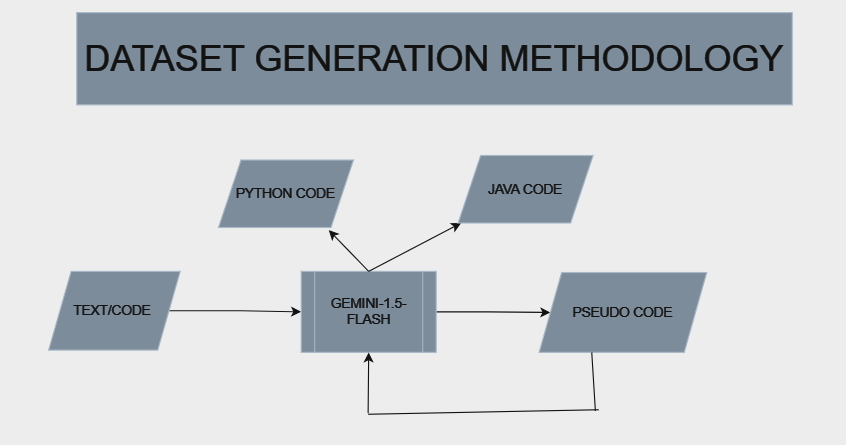
\includegraphics[width=0.7\textwidth]{dataset_methodology.png} % Replace with actual flowchart file
\caption{Dataset Generation Methodology}
\label{fig:dataset-methodology}
\end{figure}

\subsubsection{Algorithms}

The process of data preparation is done through several key steps to ensure the quality of the generated data as being both balanced and effective. We integrate the \textit{Gemini API}, which creates structured API calls that transform pseudocode into corresponding code snippets, starting with Java and Python code generation from pseudocode instructions. Next, we \textit{balance the data} so that we have equal numbers of pairs of Java and Python code by keeping the dataset fair to allow for cross-language training. Last but not least, we implement a 4-second delay between requests in order not to hit \textit{API rate limits}. That's essential to avoid hitting any breaks during the process. These steps combined result in a dataset that is reliable, well-rounded, and ready for further use.

\begin{algorithm}
\caption{Generate Balanced Code Pairs from Text Input}
\label{alg:balanced_code_pairs}
\begin{algorithmic}[1]
\Require Two CSV files: \texttt{xlcost\_text\_to\_code.csv}, \texttt{Dataset.csv}
\Ensure \texttt{Dataset.csv} updated with balanced and effective code pairs

\State Load data from \texttt{xlcost\_text\_to\_code.csv} and \texttt{Dataset.csv}
\State Configure API key and initialize the Generative AI model
\State Determine the total number of rows in the dataset, $n$
\For{each text sample in \texttt{data["text"][1:n]}}
    \State \textbf{Generate pseudocode} using the text input
    \State \textbf{Generate Python code} from the pseudocode
    \State \textbf{Generate Java code} from the pseudocode
 
    \State Structure the generated data into a new DataFrame
    \State Append the new DataFrame to the existing dataset
    \State Save the updated dataset to \texttt{Dataset.csv}
\EndFor
\State \textbf{Output:} Updated \texttt{Dataset.csv}
\end{algorithmic}
\label{alg:generate-balanced-code}
\end{algorithm}

Generative AI, for example, Google Gemini-1.5 \cite{gemini2023}, makes use of advanced large-scale language models trained on multiple datasets to process natural language prompts and generate programmatic code in multiple languages. The technology allows for context-aware mechanisms to be used for accurate and versatile code generation. For data handling, the system uses Pandas, a Python-based data manipulation library to efficiently read, update, and save datasets in structured formats like.csv. It offers concatenation and indexing functionalities that can append newly created outputs including pseudo-code, Python and Java code into the system iteratively. This approach to workflow automation allows more scalability and consistency across different prompts. Moreover, for cross-language compatibility, this model designs its prompts such that they do not rely on the built-in functions that exist in other languages, allowing easy translations across languages.

The self-attention mechanism is a fundamental component of the transformer architecture, computing relative relationships between input tokens as shown in equation \ref{eq:self-attention}:

\begin{equation}
\text{Self-Attention}(Q, K, V) = \text{softmax}\left(\frac{QK^\top}{\sqrt{d}}\right)V
\label{eq:self-attention}
\end{equation}

where \( Q \) (query), \( K \) (key), and \( V \) (value) matrices are derived from input embeddings through learned transformations. The scaling factor \( \sqrt{d} \) stabilizes softmax probabilities, focusing computational resources on the most relevant tokens. Layer normalization further stabilizes model training by normalizing input vectors through the formula, as expressed in equation \ref{eq:layer-norm}:

\begin{equation}
\text{Norm}(x) = \frac{x - \mu}{\sigma + \epsilon}
\label{eq:layer-norm}
\end{equation}

where \( \mu \) is the mean, \( \sigma \) is the standard deviation, and \( \epsilon \) is a small constant for numerical stability. The feedforward layers in transformers enhance the model’s non-linear learning capacity, expressed as shown in equation \ref{eq:ffn}:

\begin{equation}
\text{FFN}(x) = \text{max}(0, xW_1 + b_1)W_2 + b_2
\label{eq:ffn}
\end{equation}

where \( W_1 \), \( W_2 \) are weight matrices, and \( b_1 \), \( b_2 \) are bias vectors. Lastly, cross-entropy loss optimizes the model by minimizing the error between true labels (\( y_i \)) and predictions (\( \hat{y}_i \)) using the formula in equation \ref{eq:cross-entropy}:

\begin{equation}
L = -\sum_{i=1}^N y_i \log(\hat{y}_i)
\label{eq:cross-entropy}
\end{equation}

These interconnected methodologies ensure the system’s robustness and precision in generating cross-compatible, efficient programmatic solutions.


The process begins with feeding a set of text instructions into the Gemini model to generate pseudocode, an abstract, language-agnostic representation of the program's logic. The pseudocode is then fed again into Gemini to produce executable code snippets in both Java and Python. This ensures that the generated code snippets remain independent of specific language attributes or properties, such as Python's \texttt{.reverse()} method. This is done to make the output more versatile and compliant with wider standards of programming; that it is not dependent on specific inbuilt functions or language syntaxes. Through this two-stage process, the method ensures production of modular, efficient, and language-independent code.



One of the main challenges during implementation was that there was an imbalance between the pseudocode instructions and significant differences in syntax and semantics between Java and Python. The approach to this was a balanced dataset, where the number of Java and Python snippets were equal to each other for consistency and compatibility. The other challenge was that API rate limits could break up iterative workflows. This problem was solved by incorporating a delay mechanism between API calls, thus making sure the system respects rate constraints while executing uninterruptedly.

\subsubsection{Pre-training Objective}
A denoising goal named \textit{span corruption} is used to pre-train the T5 model. This configuration substitutes a unique token for randomly masked text passages. Reconstructing the original text is the aim of the model. Mathematically, let \( \hat{X} \) be the corrupted input and \( X \) the original sequence, then the objective is to maximize the formula in equation \ref{eq:pretrain-objective}:

\begin{equation}
\mathcal{L}_{\text{pretrain}} = \sum_{i=1}^n \log P(x_i | \hat{X}, \theta)
\label{eq:pretrain-objective}
\end{equation}
where \( \theta \) represents the model parameters.


\begin{algorithm}
\caption{Training and Evaluation of a Code Translation Model}
\label{alg:code_translation}
\begin{algorithmic}[1]
\Require 
\begin{itemize}
    A pre-trained T5 transformer model.
    A parallel dataset of Java and Python code samples.
\end{itemize}
\Ensure A fine-tuned model capable of translating Java code to Python.

\State \textbf{Step 1: Model Initialization}

Load a pre-trained T5 transformer as the base translation model.

Configure the model for the specified hardware (e.g., GPU or CPU).

\State \textbf{Step 2: Data Preparation}

Retrieve the dataset containing Java code and corresponding Python translations.

Split the dataset into training and validation subsets

\State \textbf{Step 3: Model Fine-Tuning}

Define the loss function to minimize translation error

Optimize hyperparameters such as batch size, learning rate, and number of epochs.

\State \textbf{Step 4: Evaluation}

Evaluate the fine-tuned model on the validation dataset using metrics BLEU.

\State \textbf{Step 5: Inference}

Provide the fine-tuned model with unseen Java code samples.

Generate Python translations for the input samples.

Analyze the outputs qualitatively and quantitatively.

\State \textbf{Step 6: Model Deployment} 

Save the fine-tuned model and tokenizer to a persistent storage system for future inference and experimentation.

\end{algorithmic}
\end{algorithm}

\section{Results and Analysis}

\subsection{Dataset Statistics} The final dataset contains 667 rows, each representing a pseudocode instruction alongside its semantically equivalent Java and Python implementations. This structured dataset serves as the foundation for training and evaluating the T5-based code translation model. As noted earlier, the pseudocode column was not used in training, but only for prompts to Gemini API, which generated the corresponding Java and Python program snippets.

\begin{table}[h!]
\centering
\caption{Sample code snippets in a table} % Caption at the top
\label{tab:code-snippets}
\adjustbox{max width=\textwidth}{ % Scale table to fit within page width
\small % Reduce font size for the whole table
\begin{tabular}{|c|c|c|}
\hline
\textbf{Pseudocode} & \textbf{Java Snippet} & \textbf{Python Snippet} \\
\hline
\begin{minipage}[t]{0.3\textwidth}
\begin{lstlisting}[basicstyle=\ttfamily\scriptsize, breaklines=true]
Maximum Prefix Sum possible by merging two given arrays;
Java Program to implement the above approach;
Stores the maximum prefix sum of the array A[];
Traverse the array A[]
Stores the maximum prefix sum of the array B[];
Traverse the array B[];
\end{lstlisting}
\end{minipage}
&
\begin{minipage}[t]{0.3\textwidth}
\begin{lstlisting}[language=Java, basicstyle=\ttfamily\scriptsize, breaklines=true]
public static int maxPrefixSum(int[] A, int[] B) {
    int maxPrefixSumA = 0, maxPrefixSumB = 0;
    for (int i = 0; i < A.length; i++) {
      maxPrefixSumA = Math.max(maxPrefixSumA, maxPrefixSumA + A[i]);
    }
    for (int i = 0; i < B.length; i++) {
      maxPrefixSumB = Math.max(maxPrefixSumB, maxPrefixSumB + B[i]);
    }
    return Math.max(maxPrefixSumA, maxPrefixSumB);
  }
\end{lstlisting}
\end{minipage}
&
\begin{minipage}[t]{0.3\textwidth}
\begin{lstlisting}[language=Python, basicstyle=\ttfamily\scriptsize, breaklines=true]
def max_prefix_sum(A, B):
  max_prefix_sum_A = 0
  for i in range(len(A)):
    max_prefix_sum_A = max(max_prefix_sum_A, max_prefix_sum_A + A[i])
  max_prefix_sum_B = 0
  for i in range(len(B)):
    max_prefix_sum_B = max(max_prefix_sum_B, max_prefix_sum_B + B[i])
  return max(max_prefix_sum_A, max_prefix_sum_B)
\end{lstlisting}
\end{minipage}
\\
\hline
\begin{minipage}[t]{0.3\textwidth}
\begin{lstlisting}[basicstyle=\ttfamily\scriptsize, breaklines=true]
Ways to remove one element from a binary string so that XOR becomes zero |
Java program to count number of ways to remove an element so that XOR of remaining string becomes 0. ;
Returns number of ways in which XOR become ZERO by remove 1 element ;
Counting number of 0 and 1 ;
If count of ones is even then return count of zero else count of one ;
\end{lstlisting}
\end{minipage}
&
\begin{minipage}[t]{0.3\textwidth}
\begin{lstlisting}[language=Java, basicstyle=\ttfamily\scriptsize, breaklines=true]
public static int countWays(String str) {
    int count0 = 0;
    int count1 = 0;
    for (int i = 0; i < str.length(); i++) {
      if (str.charAt(i) == '0') {
        count0++;
      } else {
        count1++;
      }
    }
    if (count1 % 2 == 0) {
      return count0;
    } else {
      return count1;
    }
  }
\end{lstlisting}
\end{minipage}
&
\begin{minipage}[t]{0.3\textwidth}
\begin{lstlisting}[language=Python, basicstyle=\ttfamily\scriptsize, breaklines=true]
def count_ways(s):
  count_zero = s.count('0')
  count_one = s.count('1')
  if count_one % 2 == 0:
    return count_zero
  else:
    return count_one
\end{lstlisting}
\end{minipage}
\\
\hline
\end{tabular}
}
\end{table}

The dataset, shown in Table \ref{tab:code-snippets}, serves as a fundamental resource for training and evaluating the T5-based model. It contains various examples of pseudocode, Java, and Python code snippets used for translation tasks.

\begin{table}[h!]
\centering
\caption{Performance of T5 model on benchmark dataset.} % Caption at the top
\label{tab:bleu_results}
\begin{tabular}{|c|c|c|}
\hline
\textbf{Model} & \textbf{Metric} & \textbf{Score}\\
\hline
T5-small & BLEU & 42 \\
\hline
\end{tabular}
\end{table}

The BLEU score for the T5 model, as presented in Table \ref{tab:bleu_results}, indicates that the model performs reasonably well in translating code from Java to Python, but there is still room for improvement.

\begin{table}[h!]
\centering

\caption{Java to Python Code Snippets}
\label{table:code_snippets_java_python}
\adjustbox{max width=\textwidth}{ % Scale table to fit within page width
\small % Reduce font size for the whole table
\begin{tabular}{|c|c|}
\hline
\textbf{Java Snippet} & \textbf{Python Snippet} \\
\hline
\begin{minipage}[t]{0.45\textwidth}
\begin{lstlisting}[language=Java, basicstyle=\ttfamily\scriptsize, breaklines=true]
public int sum(int a, int b) {
        return a + b;
    }
\end{lstlisting}
\end{minipage}
&
\begin{minipage}[t]{0.45\textwidth}
\begin{lstlisting}[language=Python, basicstyle=\ttfamily\scriptsize, breaklines=true]
def sum(a, b):
    return a + b

return sum(a, b)
\end{lstlisting}
\end{minipage} \\
\hline
\end{tabular}
}
\end{table}

Table \ref{table:code_snippets_java_python} demonstrates some simple Java to Python code translations, highlighting the syntax similarities and differences between the two languages.

\textit{Key Advantage}: 
The framework offers several notable advantages. First, it ensures high-quality translations, leveraging the capabilities of the Gemini API to deliver accurate and reliable outputs. Additionally, it is designed for scalability, allowing seamless extension to support other programming languages as needed. Furthermore, the framework accommodates both semantic and syntactic variability, making it versatile and effective for diverse use cases in code transpilation.


The BLEU score, a commonly used metric for sequence-to-sequence tasks, was used to assess the T5 model's performance. Table \ref{tab:bleu_results} displays the findings.

\section{Conclusion and Future Work}

The findings indicate that the T5 model demonstrates the potential to produce reasonable quality translations from Java to Python, achieving a BLEU score of 42. While this score suggests room for improvement, it highlights that the generated translations are a solid starting point. An experienced programmer can refine these outputs more efficiently than performing a full manual transpilation, significantly saving time and effort. Future research could focus on testing alternative models for Java-to-Python transpilation to enhance performance, exploring the feasibility of T5 and other models for transpilation across a broader range of programming languages, and applying the T5 model to low-resource programming languages to evaluate its adaptability and efficiency in diverse and challenging linguistic contexts. These efforts could pave the way for the development of more robust and efficient automated programming tools.

\bibliographystyle{plain}
\bibliography{references}

\end{document}
